% section 2
% Kota Miura (miura@embl.de)

\section{Intensity}

An image has only one type of information: a distribution of intensity. The image analysis in biology deals with this distribution in quantitative ways. We investigate the distribution from different angles using various algorithms and analyze biological phenomena such as shapes, cell movements and protein-protein interactions. For example in GFP labeled cells, intensity of signal is directly related to the density of the labeled biological component.
We now start studying how to interpret signals, and how to extract biologically meaningful numerical values out of intensity distribution. 

\subsection{Histogram}
\label{subsec:histogram}

If there is an 8-bit image with 100 pixel width and 100pixel height,
there are 10,000 pixels. Each of these pixels has certain pixel value.
Intensity histogram of an image is a plot that shows distribution of pixel counts over a range of pixel values, 
typically its bit depth or between the minimum and the maximum pixel value with in the image. 
Histogram is useful for examining the signal and
background pixel values for determining a threshold value to do segmentation.
We will study image threshold in \ref{sec:segmentation}). 


\begin{indentexercise}{1}
Open \textbf{Cell-Colony.tif}. Do
\ijmenu{[Analyze > Histogram]}. A new window appears. The
x-axis of the graph is pixel value. Since the image bit-depth is 8-bit,
the pixel values ranges from 0 to 255. The y-axis is the number of
pixels (so the unit is [count]). Since 255 = white and 0 = black, the
histogram has long tail towards the lower pixel value. This reflects
the fact that the image has white background and black dots.

Check pixel values in the histogram by placing the mouse pointer over
the plot and move it along the x axis. Pixel count appears at the
bottom of the histogram window. Switch to the cell colony image, and
place the pointer over dark spot. Read the pixel value there, and then
try finding out the number of pixels with the same value in the
histogram. What is the range of pixel values which corresponds to the
spot signal?  
\end{indentexercise} 
Histogram could also be used for enhancing contrast of image. Several
different algorithms are available for this: histogram normalization,
histogram equalization and local histogram normalization. 

If the histogram is occupying only part of the available dynamic range
of image bit depth (8-bit: 0 -- 255, 16-bit: 0 -- 65535), we could
adjust pixel values of image to increase its range so that contrast become more
enhanced. There are two ways to do this: normalization and
equalization. 

\subsubsection{Normalization}

With normalization, pixel values are normalized according to the
minimum and the maximum pixel values in the image and bit-depth. If the minimum pixel value is
\textit{pmin} and the maximum is \textit{pmax} in an 8-bit image, then normalization is done as follows:

\begin{equation*}
\mathit{NewPixelValue}=\frac{(\mathit{OriginalPixelValue}-\mathit{pmin})}{(\mathit{pmax}-\mathit{pmin})}\ast
255
\end{equation*}

\subsubsection{Equalization}

Equalization converts pixel values so that the values are distributed
evenly within the dynamic range. Instead of describing this in detail
using math formula, I will explain it with a simple example (see Fig. \ref{fig:equalizationSimple}). 
We consider an image with its pixel values ranging
between 0 and 9. We plot the histogram from this image, the result looks
like in the figure \ref{fig:img30}. For equalization, a cumulative
plot is first prepared from such histogram. This cumulative plot is computed by progressively integrating the histogram values (see 
Fig. \ref{fig:img31}, black curve).
To equalize (flatten) the pixel intensity distribution within the range 0-9, we would ideally require a straight diagonal
cumulative plot (in other words, the probability density of the 
pixel intensity distribution should be near-flat). To get such plot, we need to compensate the histogram by shifting values from the bars 5 and 7 to the bars 7 and 9, respectively (now, bars are in
red after shifting). After this shifting the cumulative plot now looks
more straight and diagonal (Fig. \ref{fig:img31} right, red curve).


%double figure
\begin{figure}[H]
 \centering
 \subfloat[]{\label{fig:img30}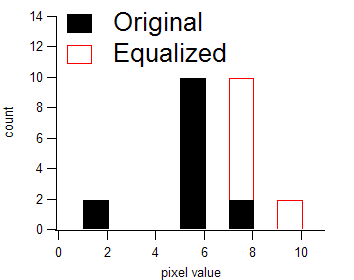
\includegraphics[height = 45mm]{fig/CMCIBasicCourse201102-img30.png}}
 \subfloat[]{\label{fig:img31}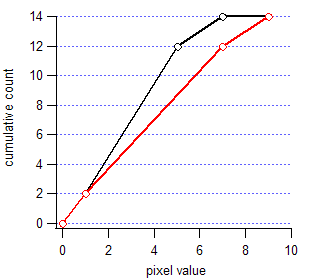
\includegraphics[height = 45mm]{fig/CMCIBasicCourse201102-img31.png}}
 \caption{ (a) Histogram Equalization: Very simple case.
The actual calculation uses cumulative plots (b) of the histogram of original
image, and uses it as a look up table to convert original pixel value,
applied point-by-point. }
 \label{fig:equalizationSimple}
\end{figure}

\begin{indentexercise}{2}
Histogram Normalization and Equalization:
\item Open sample image \textbf{g1.tif}, and then duplicate the image by
\ijmenu{[Image > Duplicate]}. Click the duplicate and then \ijmenu{[Image > Process > Enhance Contrast]}. A dialog window pops up. Set "Saturated Pixels" to 0.0\% and check "Normalize", while unchecking "Equalize Histogram", then click OK.
Compare histogram of original and normalized images .  

\item Duplicate g1.tif again by \ijmenu{[Image > Duplicate]}. Click the
duplicate and then \ijmenu{[Image > Process > Enhance Contrast]}. A dialog window pops up. Set "Saturated
Pixels" to 0.0\% and uncheck "Normalize", while check "Equalize Histogram", then click OK.
Compare histogram of original, normalized and equalized images
(\ijmenu{[Analyze > Histogram]}).

\end{indentexercise}

\begin{indentexercise}{3}
Local Histogram Equalization (Optional):
\item Histogram equalization could also be performed on a local basis. This becomes
powerful, as more local details could be contrast enhanced. You could
try this with the same image g1.tif, by \ijmenu{[Pligins > CMCICourseModules > CLAHE]} 
(if you have installed the course plugin in ImageJ) or if you are using Fiji, \ijmenu{[Process > Enhance Local Contrast (CLAHE)] }
\end{indentexercise}



\subsection{Region of Interest (ROI) }
\label{subsec:roi}
To apply certain operation to a specific part of the image, you can
select a region by "region of interest
(ROI)" tools. The shape of the ROI could be various,
such as rectangular, elliptical, polygon, free hand or a line
(straight, segmented or free hand). There are several functions that
will be used often in association with ROI tools. 

\begin{indentexercise}{1}
Cropping. Open any image. Select a region by
rectangular ROI. Then \ijmenu{[image > Crop]}. This will
remove the unnecessary part of the image, to reduce calculation time.
\end{indentexercise}

\begin{indentexercise}{2}
Masking. Open any image. Select a region by
rectangular ROI. Then \ijmenu{[Edit > clear]} followed by
\ijmenu{[Edit > Clear Outside]}. After checking what
happened, do \ijmenu{[Edit Fill]}. (same operation could
be done by \ijmenu{[Edit > Selection > Create Mask]})
\end{indentexercise}

\begin{indentexercise}{3}
Invert ROI. Open any image. Select a region by
rectangular ROI. Then\ijmenu{ [Edit > Selection > Make Inverse]}. In this way, you can select region
excluding the region you initially selected.
\end{indentexercise}

\begin{indentexercise}{4}
Redirecting ROI. Open any two images. In one
of the image, select a region by rectangular ROI. Then activate the
other image by clicking that window, and do \ijmenu{[Edit > Selection > Restore Selection]}. ROI with
same size and position will be reproduced in the window. 
\end{indentexercise}



\begin{indentexercise}{5}
ROI manager. You can store the position and
size of the ROI in the memory. Select a region by rectangular ROI.
\ Then \ijmenu{[Analysis > Tools > Roi Manager]}. Click "Add" button to store
ROI information. Stored ROI can be saved as a file, and could be loaded
again when you restart the ImageJ.
\end{indentexercise}


\subsection{Intensity Measurement}

As you move the mouse pointer over individual pixels, their intensity value are indicated in the ImageJ menu bar. This is the easiest way to
read pixel intensities, but you can only get the values one by one. Here we learn a way to get statistical information of a group
of pixels within ROI. This has more practical usages for research. 

To measure pixel values of a ROI, ImageJ has a function \ijmenu{[Analyze >
Measure]}. Before using this function, you could specify the parameters 
you want to measure by \ijmenu{[Analyze > Set measurements]}. There are many parameters
in the "Set measurement" window. Details on these parameters are listed in the
Appendix \ref{app2}. For intensity measurements the following parameters are
important.


\begin{itemize}
\item \textbf{Mean Gray Value} - Average gray value within the selection. This
is the sum of the gray values of all the pixels in the selection
divided by the number of pixels. Reported in calibrated units (e.g.,
optical density) if Analyze/Calibrate was used to calibrate the image.
For RGB images, the mean is calculated by converting each pixel to
grayscale using the formula $gray=0.299red+0.587green+0.114blue$ or the
formula $gray=(red+green+blue)/3$ if "Unweighted RGB to
Grayscale Conversion" is checked in Edit/Options/Conversions.

\item\textbf{Standard Deviation}{}- Standard deviation of the gray values.

\item\textbf{Min \& Max Gray Level} - Minimum and maximum gray values within
the selection.

\item\textbf{Integrated Density} - The sum of the values of the pixels in the
image or selection. This is equivalent to the product of Area and Mean
Gray Value. The Dot Blot Analysis example demonstrates how to use this
measurement to analyze a dot blot assay.
\end{itemize}

A short note on image-based fluorometry: In biochemical experiments,
scientists measure protein concentration by measuring absorbance of UV
light or by labeling proteins with dyes or fluorescence and measure the
intensity of emission. This is because light absorbance or the
intensity of fluorescence intensity is proportional to the density of
protein in the irradiated volume within cuvette. Very similar to this
when fluorescence image of cells are taken, pixel values (which is the
fluorescence intensity) are proportional to the density of the labeled
protein at each pixel positions. For this reason, measurement of
fluorescence intensity using digital imaging could be considered as the
two dimensional version of the conventional fluorometry. 

\begin{indentexercise}{1}
\item Open a sample image \textbf{cells\_Actin.tif}. Before actually executing the measurement,
do \ijmenu{[Analyze > Set Measurements]}. A dialog
window opens. There are many parameters listed in the upper-half of the
window.

%figure
\begin{figure}[htbp]
\begin{center}
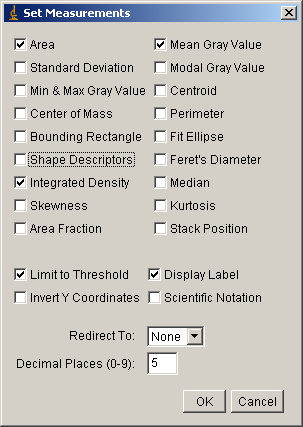
\includegraphics[width=8.017cm,height=11.298cm]{fig/CMCIBasicCourse201102-img32.png}
\caption{Set Measurements Window}
\label{fig:img32}
\end{center}
\end{figure}


The parameters we select now are:
\begin{itemize}
\item Area
\item Integrated Density 
\item Mean Gray Value
\end{itemize}

Check the box of these three parameters. Integrated density is the sum
of all the pixel values and Mean Gray Value is the average of all the
pixel values within ROI. So 

$Integrated Density = Area * Mean Gray Value$

Select one of the cells in cell\_Actin.tif image and zoom it up
using magnifying tool. Switch the tool to
"Polygon" tool. Draw polygon ROI around
the cell. Then do \ijmenu{[Analyze > Measure]}. A window
titled "Results" pops-up, listing the
measured values. Check that the integrated density is the
multiplication of area and the mean gray value.




%double figure
\begin{figure}[htbp]
 \centering
 \subfloat[]{\label{fig:img33}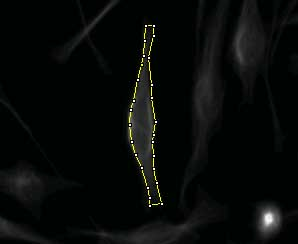
\includegraphics[height=4cm]{fig/CMCIBasicCourse201102-img33.jpg}}
 \subfloat[]{\label{fig:img34}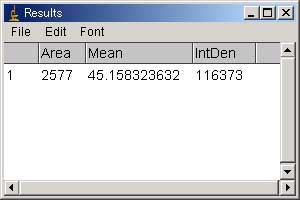
\includegraphics[height=4cm]{fig/CMCIBasicCourse201102-img34.jpg}}
 \caption{ (a) Tracing Cell Edge by Segmented ROI and Measuring the Intensity within selected area. }
 \label{fig:CellIntensityMeasurement}
\end{figure} 

This value is not the actual intensity of the fluorescence within the
cell since it also includes the background intensity (offset).
Measure the background intensity by creating a new ROI in the area
where there is no cell.

%figure
\begin{figure}[htbp]
\begin{center}
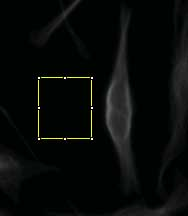
\includegraphics[height=4.5cm]{fig/CMCIBasicCourse201102-img35.jpg}
\caption{Measurement of Background}
\label{fig:img35}
\end{center}
\end{figure}

\end{indentexercise}

NOTE: When no ROI is active (no yellow bounding rectangle or so),
then the measurement is performed on the whole image.

\subsection{Image transformation: Enhancing Contrast}
\label{subsec:enhancecontrast}
Some of you might already have experience with the contrast enhancing of
digital images, since in most of imaging software like the ones that
come with digital cameras usually have this function. Low contrast images
have small difference in the tones and the objects are difficult to observe.
If the contrast is too high, then the tone difference is so much that
the picture is "over exposed".
Adjustment of contrast controls the tone difference to optimize the
visual resolution. The contrast enhancement primarily changes the LUT,
so that the original image data is unaffected (you will see in the
following exercise). The original data is changed only when you click
"Apply" button. Then the pixel values
are re-scaled according to the LUT you set.



Care must be taken for contrast enhancement since pixel values are
altered. This could be regarded as
"fraud" or
"manipulation" in science, especially if
you are measuring image intensity. If all images that you are trying to
compare were equally contrast enhanced,
then the images could eventually be compared. Even then, there will be another
pit-fall if you artificially saturate the image: this happens often
especially in the case of low bit-depth images. 

\begin{indentexercise}{1}
Open image gel\_inv.tif. Do \ijmenu{[Image > Adjust > Brightness/Contrast]}. 
Pop-up window appears which looks like the
figure below (left). The graph shown in the upper part of the window is 
the
histogram of the image just like you have seen in section \ref{subsec:histogram}. 
Since the image is 8-bit, scale in the x axis is 0 to 255.
There is also a black diagonal line. This corresponds to the LUT of the
image on the screen: pixel values in x is translated into the gray
value on the screen (brightness on the screen is y-axis). 

The slope and position of the LUT can be altered by clicking and dragging
four sliding bars under the graph, each with the name minimum, maximum,
brightness and contrast. Try changing these values and studying the
effect on the image. 

QUESTION: What is the problem with the adjustment shown in the
right side of the figure below?

%double figure
\begin{figure}[htbp]
 \centering
 \subfloat[]{\label{fig:img36}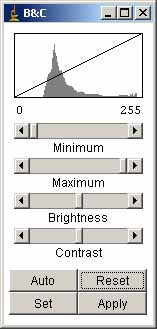
\includegraphics[width=2.762cm,height=5.803cm]{fig/CMCIBasicCourse201102-img36.jpg}}
 \subfloat[]{\label{fig:img37}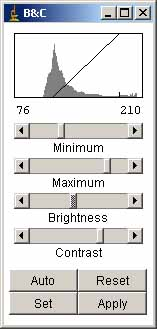
\includegraphics[width=2.762cm,height=5.803cm]{fig/CMCIBasicCourse201102-img37.jpg}}
 \caption{ (a) Histogram of \textbf{gel\_inv.tif} before enhancing contrast. (b) Some bad adjustments example. }
 \label{fig:quizEnhanceContrast}
\end{figure} 

\end{indentexercise}

\begin{indentexercise}{2}
Continued from above: the original image file
is not changed at this stage. When you push the
"Apply" button at the bottom-right
corner, the original image is altered numerically. Try set the LUT as
you like, and push the Apply: what happened to the Histogram and the
LUT indicator? (you can always
"Undo" the "Apply" by \ijmenu{[Edit > Undo]}, 
or revert to the original file by \ijmenu{[File > Revert]}).
\end{indentexercise}

\begin{indentexercise}{3}
With RGB image, it is possible to adjust the
brightness and contrast for individual color channel. Open the image
\textbf{RGB\_cell.tif}, then do \ijmenu{[Image > Adjust > Color Balance]}. 
There is a pull-down menu to specify
the channel you want to change. Try changing different channels to
optimize the image. 
\end{indentexercise}

\subsection{Image correlation between two images: co-localization plot}

In many experiments we need to compare the
localization of two or more proteins and examine whether those proteins
are co-localized. In many cases this has been evaluated by visual
inspections. But with digital images, it is possible to evaluate the
degree of co-localization more quantitatively. This is done by plotting
a so called "co-localization
plot". To do this in ImageJ one could download a
plugin \textbf{Colocalization\_Finder}\footnote{download from \url{http://rsb.info.nih.gov/ij/plugins/colocalization-finder.html}}
and install it.

The level of colocalization could be then parametrized by using statistical
values such as Pearson's coefficient and
Mander's coefficient. These values have advantages and
disadvantages depending on the image properties. For detailed
description on these issues, refer to \citet*{BolteJM2006}.

Additional insights, pitfalls and tips on localizing spot signals could
be found in \citet{Waters2009}. This paper also provides detailed examination of the precision of dot detections. 
\clearpage

\subsection{ASSIGNMENTS}

\textbf{\sffamily
Assignment 1-2-1:}

Suppose that you have an 8-bit grayscale image showing three objects of 
distinct intensities against a bright background. What would
the corresponding histogram look like?

\textbf{\sffamily
Assignment 1-2-2: }

With image \textbf{cell\_Actin.tif}, do the measurement with 4 cells and one background in image as we did in the
exercise. This time, store ROI in ROI manager (refer to \ref{subsec:roi} Roi)
and do the measurement at once. First, you store 5 different ROI one by
one ("Add" button). Then click "Show all" button in the ROI manager.
Activate all ROI by clicking the ROI name in the list while pushing
down the SHIFT key. Then click "Measure"
button. All five ROI will be measured at once. Average the values and
describe the results in text.

\textbf{\sffamily
Assignment 1-2-3: }
\begin{enumerate}
\item Optimize the contrast of image
\textbf{m51\_8bit.tif}. Be careful not to
saturate the pixels so you don't throw away important
information in the lower pixel values. Check the histogram.
Don't close the histogram window

\item After applying the adjustment above (clicking
"Apply" button), check the histogram
again. Compare the histogram before and after. What happened? Discuss
the reason.
\end{enumerate}
